\begin{pycode}



\end{pycode}

\section{Séance 1 - Caractéristique de la bobine }

\subsection{Objectifs}

Le but de cette première séance est de caractériser le capteur de proximité inductif à travers 
l’analyse de la résistance et l'inductance de la bobine, en fonction de la distance cible-capteur 
 et de la fréquence. 

\subsection{Méthode}

\begin{enumerate}
    \item Brancher la maquette sur l'analyseur d'impédance comme montré ci-dessous (cf. fig. \ref{fig: AI});
    \item Déterminer la distance de butée et se positionner à 0.5 mm de celle-ci ;
    \item Enregistrer la mesure de l'appareil qui permet d'obtenir la résistance ainsi que l'inductance de 
    la bobine sur un intervalle de 150 kHz à 15 MHz ;
    \item Répéter l'opération par pas de 0.05 mm jusqu'à atteindre 0.90 mm ce qui totalise 9 mesures.
\end{enumerate}

\insererfigure{Images/Seance1/AnalyseurImpedance.jpg}{6cm}{analyseur d'impédance}{AI}

\subsection{Caractérisation de la bobine}

\subsubsection{Impédance}


Les mesures réalisées avec l'analyseur d'impédance ont été sauvegardées en un total
de 9 fichiers CSV, un pour chacune des distances. Chaque fichier comporte une colonne propre à
la fréquence, l'inductance et la résistance. Ainsi, il est possible de déterminer l'impédance, relative
à la fréquence, selon les 9 positions de la bobine.\\


Impédance de la bobine : 

\begin{equation}
    Z_b = R_b + j \omega L_b
\end{equation}

Avec : \\
$Z_b$, l'impédance de la bobine [$\Omega$];\\
$R_b$, la résistance de la bobine [$\Omega$];\\
$L_b$, l'inductance de la bobine;\\
$\omega$, la pulsation = $ 2 \cdot \pi \cdot f$ [rad/s] ;\\
f, la fréquence [Hz].\\

Représentations schématiques du circuit : 

\begin{figure}[H]
    \begin{minipage}[c]{.50\linewidth}
        \centering
        \rotatebox{0}{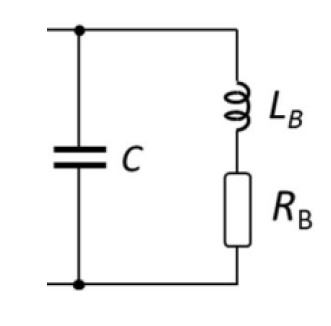
\includegraphics[scale=0.6]{Images/Seance1/Sch1.jpg}}
        \caption{Schéma électrique en série }
    \label{fig:SCH1}
    \end{minipage}
    \hfill%
    \begin{minipage}[c]{.50\linewidth}
        \centering
        \rotatebox{0}{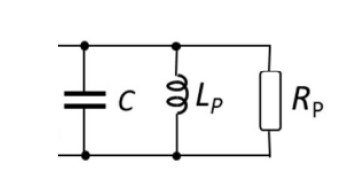
\includegraphics[scale=0.9]{Images/Seance1/Sch2.jpg}}
        \caption{Schéma électrique en parallèle }
    \label{fig:SCH2}
    \end{minipage}
\end{figure}

L'impédance ainsi déterminée a permis de représenter graphiquement l'inductance et la résistance de 
la bobine en fonction de la fréquence :


\insererfigure{Images/Seance1/Lf.png}{8cm}{Inductance en fonction de la fréquence}{Lf}
\insererfigure{Images/Seance1/Rf.png}{8cm}{Résistances en fonction de la fréquence}{Rf}

L'allure des courbes représentées sur les graphiques (cf. fig. \ref{fig: Lf} et \ref{fig: Rf})
correspondent au comportement d'un circuit RLC. Ce résultat est représentatif du montage étudié.
En effet, la \textbf{R}ésistance et est celle du fil de la bobine, l'inductance \textbf{L} est celle 
de la bobine, le \textbf{C}ondensateur est la capacité relative à la 
cible et à sa distance.\\

La fréquence de résonance du circuit peut-être aisément relevée puis-ce qu'il s'agit du passage à 0 
de l'inductance et le pic de résistance. On relève graphiquement à la 
position de repos une fréquence de résonance de 6.77 Mhz. La figure \ref{fig: Lf} montre encore
qu'à basse fréquence l'inductance est constante ce qui suggère la présence d'une cible non-ferromagnétique\\

%La figure \ref{fig: Rf} montre que les courbes se croisent à 1.63 MHz. 

%On note encore que les courbes de résistance
%se croisent à 1.62 MHz ce qui représente l'en\\


%\begin{figure}[H]
%    \begin{minipage}[c]{.50\linewidth}
 %       \centering
  %      \rotatebox{0}{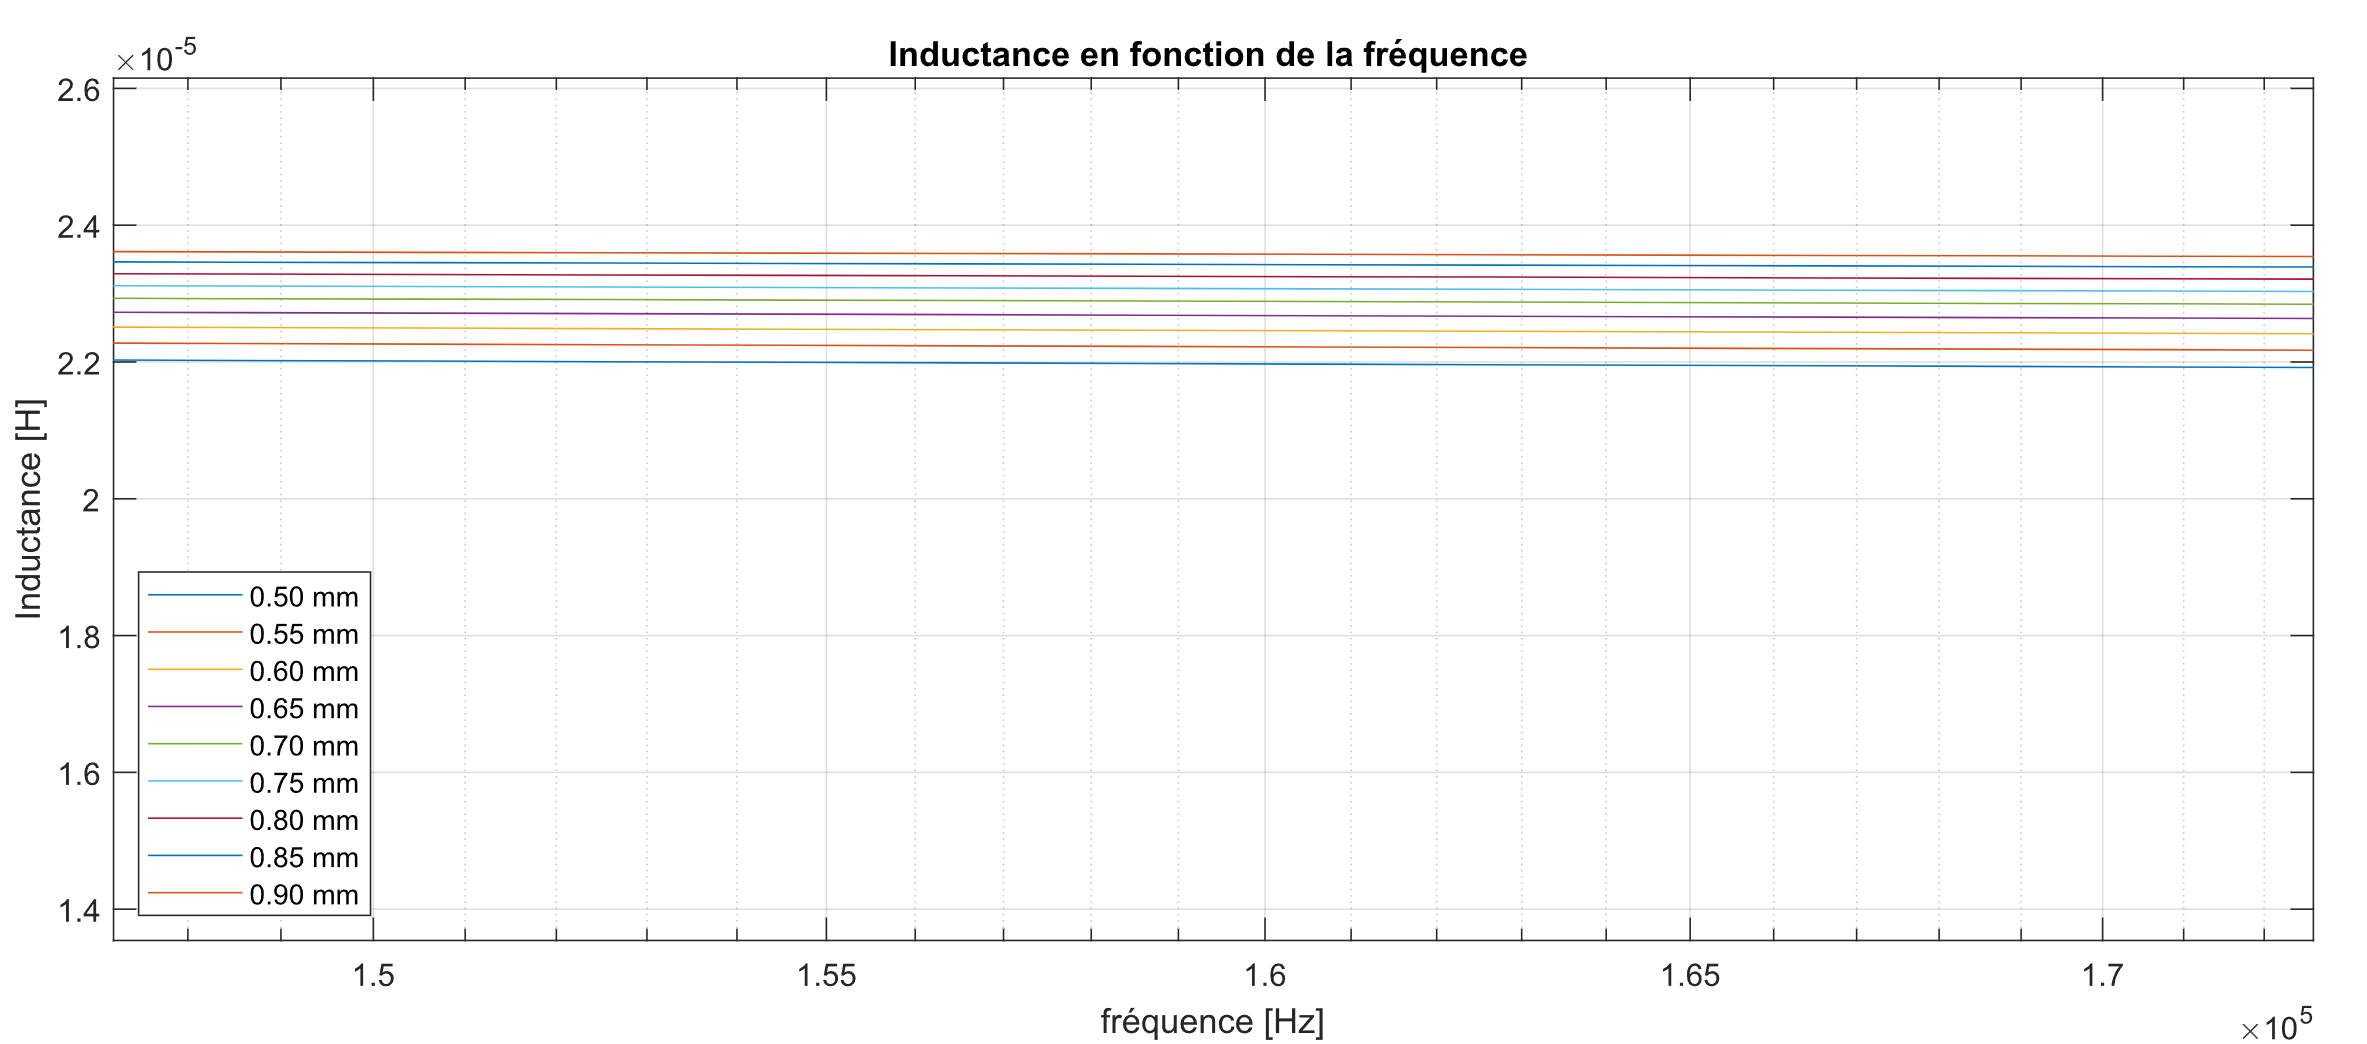
\includegraphics[scale=0.2]{Images/Seance1/zoom1L.png}}
  %      \caption{Zoom sur la figure \ref{fig: Lf}}
  %  \label{fig:SCH3}
  %  \end{minipage}
  %  \hfill%
  %  \begin{minipage}[c]{.50\linewidth}
  %      \centering
  %      \rotatebox{0}{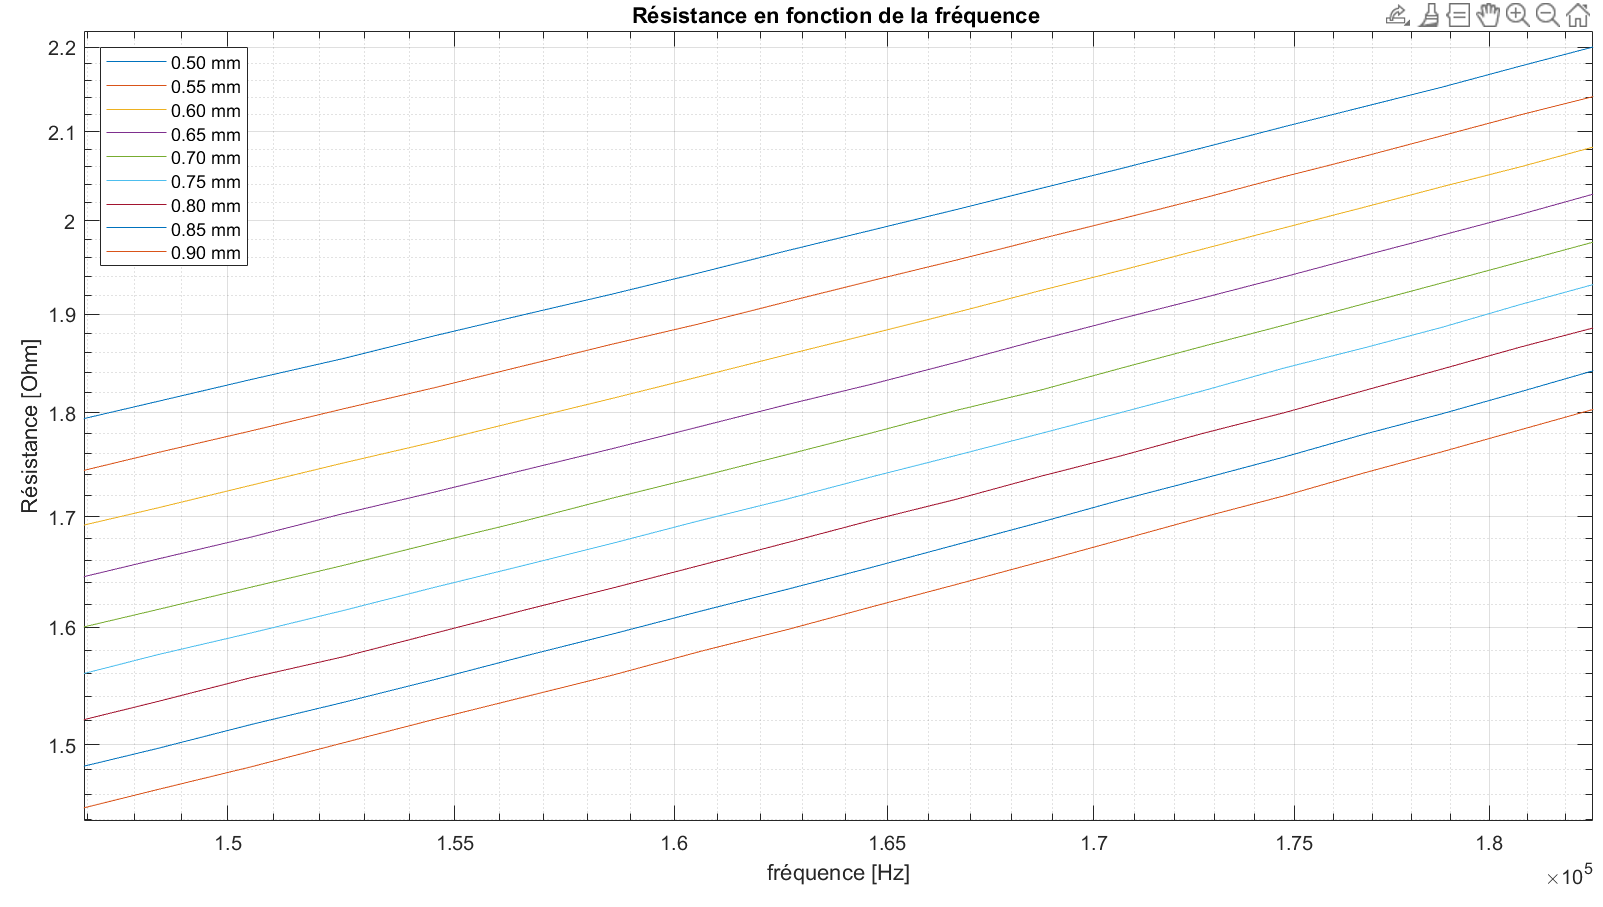
\includegraphics[scale=0.2]{Images/Seance1/zoom2R.png}}
  %     \caption{Zoom sur la figure \ref{fig: Rf}}
 %\label{fig:SCH4}
 %   \end{minipage}
%\end{figure}

Il est enfin possible de constater qu'en basses fréquences (140-160 kHz) les différentes courbes évoluent
de manière linéaire. \\





L'inductance et la résistance à 150 kHz en fonction de la distance ont ensuite été représentées :

\insererfigure{Images/Seance1/Lx.png}{8cm}{Inductance en fonction de la distance}{Lx}
\insererfigure{Images/Seance1/Rx.png}{8cm}{Résistances en fonction de la distance}{Rx}

Les courbes tracées permettent de déterminer le type de matériau de la cible, ferromagnétique ou 
non-ferromagnétique. Les figures \ref{fig: Lx} et \ref{fig: Rx} montrent une augmentation de 
l'inductance et une diminution de la résistance lors de l'éloignement de la cible ce qui correspond 
au comportement d'un matériau conducteur non-ferromagnétique. 
De plus, la cible est de couleur orangée et comportant des marques d'oxydation, ce qui permet 
de conclure qu'elle est en \textbf{cuivre}.\\  

%Les régressions réalisées (cf. fig. \ref{fig: Lx} et \ref{fig: Rx}) 


L'impédance de la bobine aux différentes distrances pour une fréquence de 150kHz à finalement été tracée :

\insererfigure{Images/Seance1/Zx.png}{8cm}{Impédance de la bobine aux distances}{Zx}

La figure \ref{fig: Zx} montre que l'impédance évolue de manière "quasi" linéaire, avec une 
variance de 0.9999. On remaque toute fois que la distance entre les point ne sont pas les mêmes. 
Plus la cible s'éloigne, plus les points se rapprochent et la sensibilité diminue (eq :\ref{eq:s}).
Ceci montre les limites de ce système, car si la sensibilité est trop faible alors les valeurs relevées
ne sont plus tolérables.
\subsubsection{Sensibilité}

Grâce aux valeurs relevées, il est également possible de déterminer la sensibilité de
ce capteur qui, pour une position de repos à 0.7 mm s'exprime : 

\begin{equation}\label{eq:s}
    \left . S_b \right |_{x=0.7} = \left . \frac{\left | \delta \underline{Z_b}\right |}{\delta x} \right |_{x=0.7}
\end{equation}

Avec: \\
$S_b$, la sensibilité [$\Omega/mm$];\\
$\delta Z$, l'écart d'impédance = $Z_{0.75} - Z_{0.65}$ [$\Omega$];\\
$\delta x$, l'écart de distance  = $x_{0.75} - x_{0.65}$ [mm].



\insererfigure{Images/Seance1/S.png}{8cm}{Sensibilité en fonction de la fréquence}{S}

Le graphique ci-dessus montre la sensibilité calculée avec l'équation \ref{eq:s} en fonction
de la fréquence, pour une position de repos de 0.7mm. Cette représentation permet d'observer
qu'un pic sensibilité se forme de 5 à 9 MHz, culminant à 21'235 [$\Omega$/mm] à la fréquence 
de 6.78 MHz. 

 
\subsection{Conclusion}

Les premières analyses de ce capteur ont donné des résultats cohérents et qui permettent
d'avoir une bonne appréhension des prochaines séances.\\

Résumer des résultats :

\begin{enumerate}
    \item Le matériau constituant la cible est le cuivre;
    \begin{itemize}
        \item Comportement conducteur non-ferromagnétique;
        \item Couleur orangée.
    \end{itemize}
    \item Pour une fréquence de 150 kHz on observe une progression linéaire de l'impédance en selon
    la position de la cible;
    \item La fréquence de résonance du capteur est de 6.78 MHz;
    \begin{itemize}
        \item Passage à 0 de l'inductance et pic de résistance (cf. fig. \ref{fig: Lf} et \ref{fig: Rx})
        \item Pic de sensibilité (cf. fig. \ref{fig: S}). 
    \end{itemize}
\end{enumerate}

